\documentclass[UTF8]{ctexbeamer}
\usetheme{Madrid}
% \usecolortheme{beaver}
\usepackage{hyperref}
\usepackage{graphicx}
\usepackage{wrapfig}
\DeclareGraphicsExtensions{.eps,.ps,.jpg,.bmp,.png}

\title{密码学入门与 Key signing party}

\author[HITLUG]{陈天宇}

\date{May 2021}

\AtBeginSection[]
{
	\begin{frame}
		\frametitle{Table of Contents}
		\tableofcontents[currentsection]
	\end{frame}
}



\begin{document}

\frame{\titlepage}
\begin{frame}
    % Table of contents 目录/大纲页
    % 自动实现对section的收集,并绘制成目录页
	\frametitle{Table of Contents}
	\tableofcontents
\end{frame}

\section{What is cryptography?}
\begin{frame}{What is Encryption \& Decryption}
    \begin{figure}
        \centering
        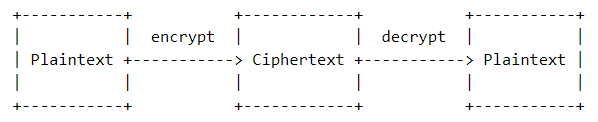
\includegraphics[width=0.8\textwidth]{encryption.png}
    \end{figure}
\end{frame}

\begin{frame}{What is cryptography?}

    The science of using mathematics to encrypt and decrypt data

    Cryptography enables you to store sensitive information or transmit it across insecure networks (like the Internet) so that it cannot be read by anyone except the intended recipient.
    
\end{frame}

\subsection{What cryptography is and what cryptography is not?}
\begin{frame}{What cryptography is and what cryptography is not?}
    \begin{itemize}
        \item Encode / Decode
        \item Encrypt / Decrypt
    \end{itemize}
\end{frame}

\begin{frame}{Encode / Decode}
    \begin{itemize}
        \item ASCII
        \item Morse code
        \item Base16 / Base32 / Base58 / Base64
        \item GB2312 / Big-5 / UTF-8
    \end{itemize}
\end{frame}

\begin{frame}{Encrypt / Decrypt}
    \begin{itemize}
        \item Conventional Encryption
        \item Symmetric-key cryptography
        \item Public-key cryptography
        \item Hybrid cryptosystem
    \end{itemize}
\end{frame}

\section{Cryptography}
\subsection{Conventional Encryption}
\begin{frame}{Conventional Encryption}
    \begin{figure}
        \centering
        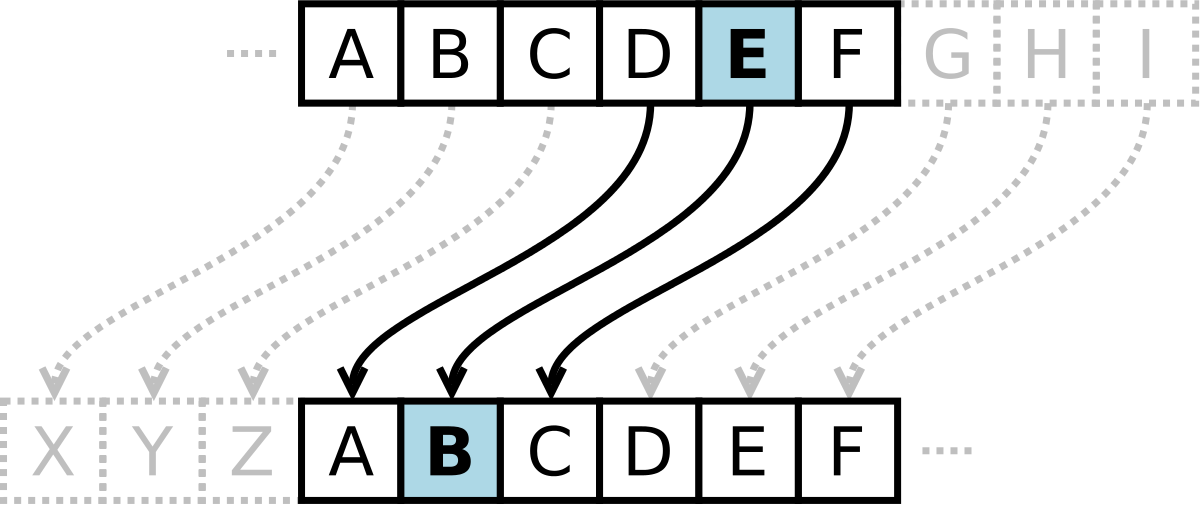
\includegraphics[width=0.8\textwidth]{caesar-cipher.png}
        \caption{凯撒密码(Caesar's Cipher)}
    \end{figure}
\end{frame}
\begin{frame}{Conventional Encryption}
    \begin{figure}
        \centering
        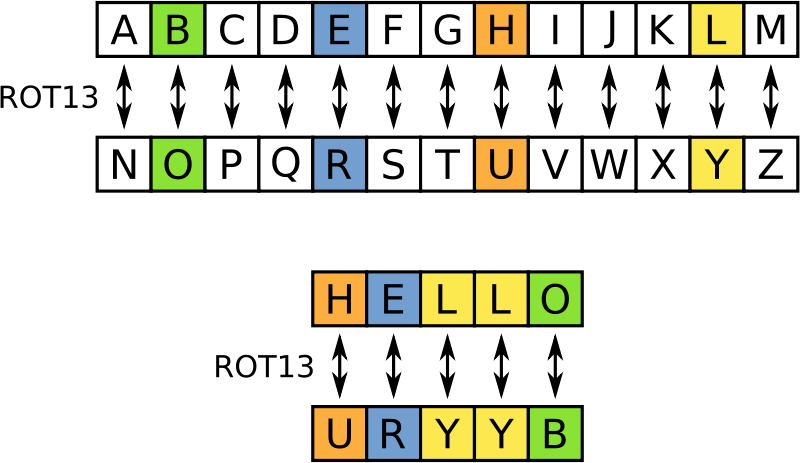
\includegraphics[width=0.8\textwidth]{rot13.png}
        \caption{ROT13}
    \end{figure}
\end{frame}
\begin{frame}{维吉尼亚密码(Vigenère cipher)}
        
    \begin{figure}
        \centering
        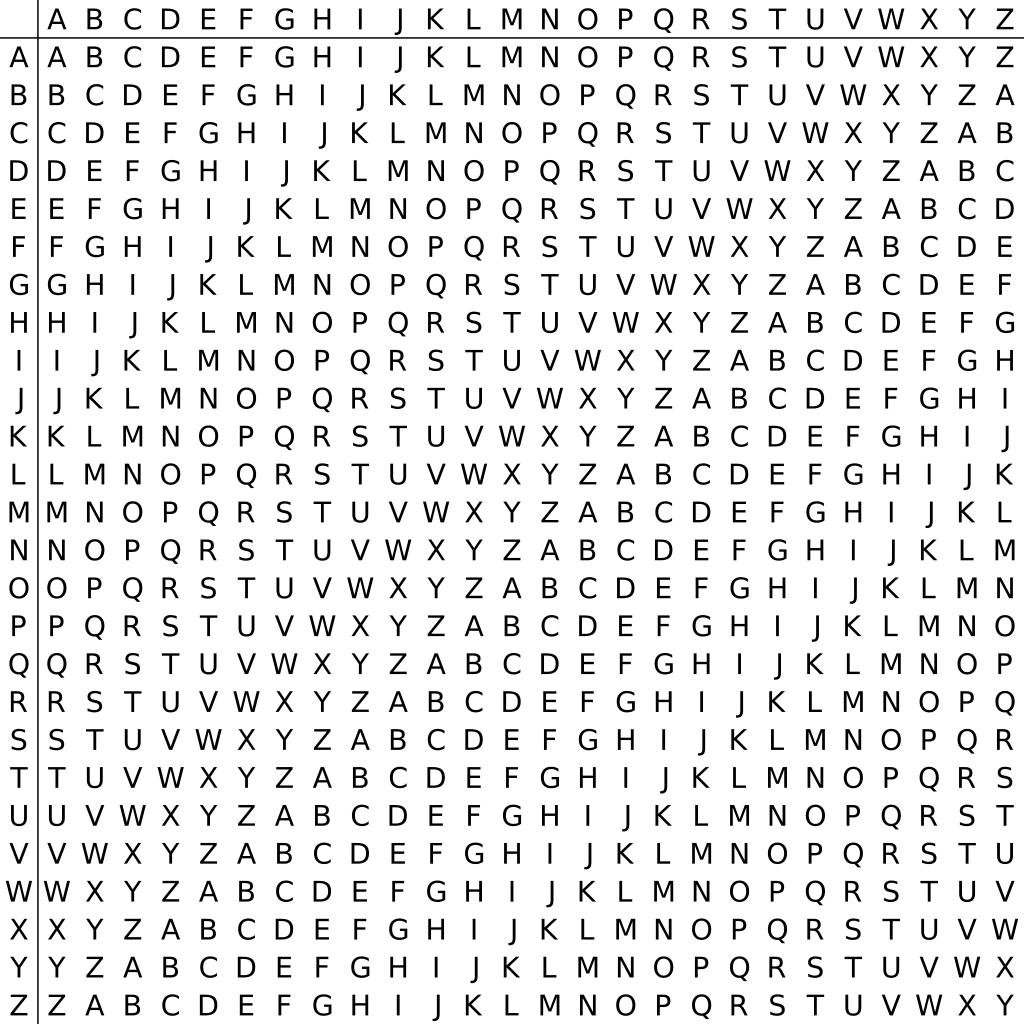
\includegraphics[width=0.5\textwidth]{vigenere.png}
        \caption{维吉尼亚密码(Vigenère cipher)}
    \end{figure}
        
\end{frame}
\begin{frame}{维吉尼亚密码(Vigenère cipher)}
    \begin{columns}
        \begin{column}{0.7\textwidth}
            \centering
            $CipherText \equiv PlainText + Key (\text{mod} 26)$
        \end{column}
        \begin{column}{0.3\textwidth}
            \begin{figure}
                \centering
                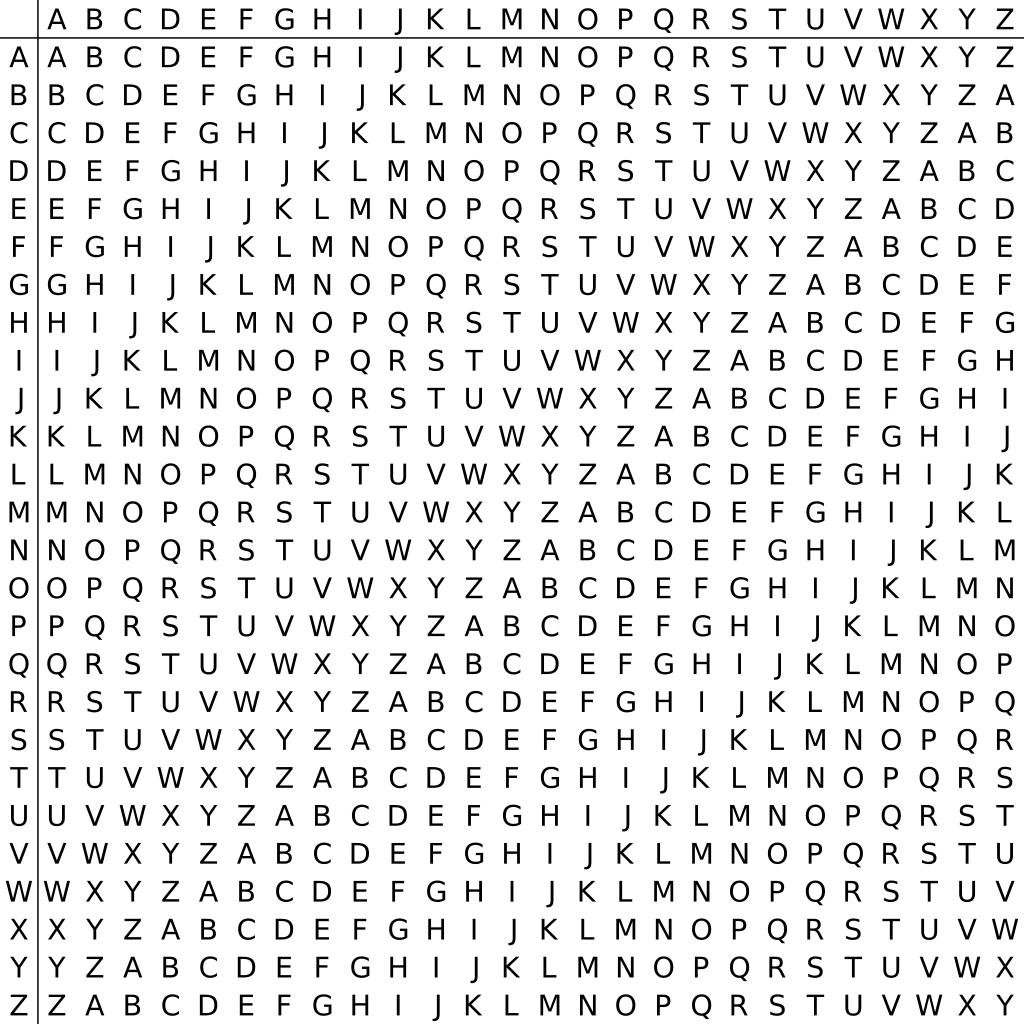
\includegraphics[width=\textwidth]{vigenere.png}
                \caption{Vigenère cipher}
            \end{figure}
        \end{column}
    \end{columns}
\end{frame}
\begin{frame}{恩尼格玛密码机(Enigma)}
    \textit{\url{https://zh.wikipedia.org/wiki/恩尼格玛密码机}}
    
    \textit{\url{https://youtu.be/V4V2bpZlqx8}}
\end{frame}
\subsection{Modern Cryptography}
\subsubsection{Symmetric-key cryptography}

\begin{frame}{Symmetric-key cryptography}
    \begin{itemize}
        \item DES
        \item 3DES
        \item AES
        \item RC2
        \item RC4
        \item Salsa20
    \end{itemize}
\end{frame}

\begin{frame}{DES}
    DES 1976年被美国联邦政府的国家标准局确定为联邦资料处理标准(FIPS),随后在国际上广泛流传开来。
    
    它基于使用56位密钥的对称算法。
    
    \pause
    
    \begin{itemize}
        \item 1998年7月,EFF的DES破解机(Deep Crack)在56小时内破解了DES密钥
        \item 1999年1月,Deep Crack和distributed.net合作在22小时15分钟内破解了一个DES密钥
        \item 1999年10月,DES作为FIPS46-3第四次延长标准期限,其中规定优先使用3DES,而普通DES只允许在遗留的系统中应用
    \end{itemize}
    
    \pause
    
    2000年10月,在历时接近5年的征集和选拔之后,NIST选择了高级加密标准(AES)替代DES和3DES。2001年2月28日,联邦公报发表了AES标准,以此开始了其标准化进程,并于2001年11月26日成为FIPS PUB 197标准。
\end{frame}
\begin{frame}{3DES}
    对每个数据块应用三次资料加密标准(DES)算法
    
    由于DES密钥长度过低,容易被暴力破解;3DES便被设计用来提供一种相对简单的方法,通过增加DES的密钥长度来避免被暴力破解,而不是设计一种全新的块密码算法。
\end{frame}

\begin{frame}{AES}
    \begin{itemize}
        \item AddRoundKey
        \item SubBytes
        \item ShiftRows
        \item MixColumns
    \end{itemize}
\end{frame}
\subsubsection{Public-key cryptography}
\begin{frame}{Public-key cryptography}
    \begin{itemize}
        \item DSA
        \item RSA
        \item ElGamal
        \item ECDSA
    \end{itemize}
\end{frame}

\begin{frame}{DSA}
    基于模算数和离散对数的复杂度
    
    NIST于1991年提出将DSA用于其数字签名标准,并于1994年将其作为FIPS 186采用。
    
\end{frame}
\begin{frame}{RSA}

    \begin{columns}
        \begin{column}{0.3\textwidth}
            $$p, q, N, r, e, d$$
        \end{column}
        \begin{column}{0.7\textwidth}
            \begin{figure}
                \centering
                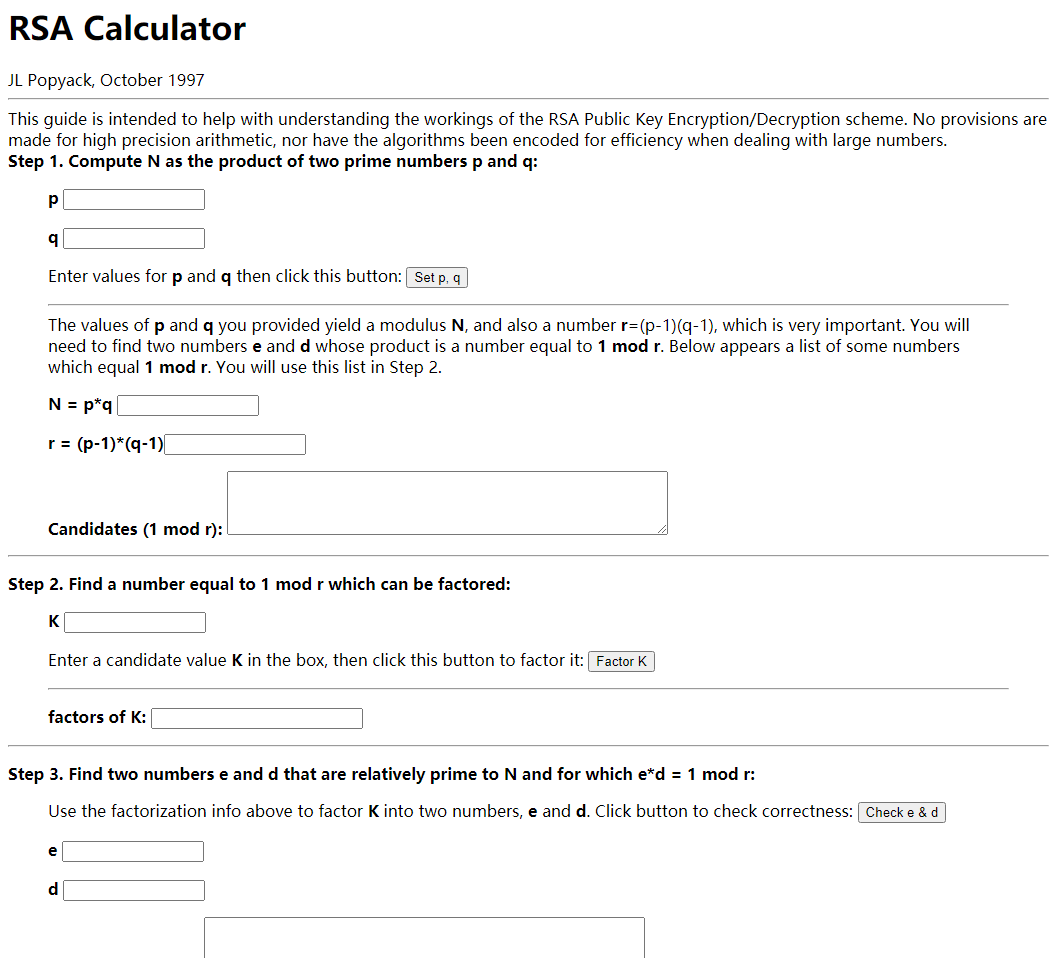
\includegraphics[width=0.7\textwidth]{rsa-calc.png}
                \caption{\href{https://www.cs.drexel.edu/~jpopyack/IntroCS/HW/RSAWorksheet.html}{RSA Calculator}}
            \end{figure}
        \end{column}
    \end{columns}
\end{frame}

\subsubsection{Hybrid cryptosystem}
\begin{frame}{Hybrid cryptosystem \& Session key}

    A hybrid cipher uses both a symmetric cipher and a public-key cipher. It works by using a public-key cipher to share a key for the symmetric cipher. The actual message being sent is then encrypted using the key and sent to the recipient. Since symmetric key sharing is secure, the symmetric key used is different for each message sent. Hence it is sometimes called a session key.
    
    \href{https://www.gnupg.org/gph/en/manual/x209.html}{Explanation in \textit{The GNU Privacy Handbook}}
\end{frame}

\subsection{国密算法}
\begin{frame}{国密算法}
    \begin{itemize}
        \item SM1:为对称加密。其加密强度与AES相当。该算法不公开,调用该算法时,需要通过加密芯片的接口进行调用。
        \item SM2:非对称加密,基于ECC(椭圆加密算法)。该算法已公开。由于该算法基于ECC,故其签名速度与秘钥生成速度都快于RSA。ECC256位(SM2采用的就是ECC256位的一种)安全强度比RSA 2048位高,但运算速度快于RSA。即SM2>RSA2048,安全度高且运算速度块。
        \item SM3:消息摘要,可以用MD5作为对比理解。该算法已公开。校验结果为256位。
        \item SM4:对称加密,密钥长度和分组长度均为128位。无线局域网标准的分组数据算法。
    \end{itemize}
\end{frame}

\begin{frame}{GmSSL}

    \textit{GmSSL是一个开源的密码工具箱,支持SM2/SM3/SM4/SM9/ZUC等国密(国家商用密码)算法、SM2国密数字证书及基于SM2证书的SSL/TLS安全通信协议,支持国密硬件密码设备,提供符合国密规范的编程接口与命令行工具,可以用于构建PKI/CA、安全通信、数据加密等符合国密标准的安全应用。GmSSL项目是OpenSSL项目的分支,并与OpenSSL保持接口兼容。因此GmSSL可以替代应用中的OpenSSL组件,并使应用自动具备基于国密的安全能力。GmSSL项目采用对商业应用友好的类BSD开源许可证,开源且可以用于闭源的商业应用。}
    
    \textit{\url{http://gmssl.org/}}
    
\end{frame}
\subsection{Hash Functions}
\begin{frame}{Hash Functions}
    \begin{itemize}
        \item MD5
        \item SHA-1
        \item SHA-2(SHA-224, SHA-256, SHA-384, etc.)
    \end{itemize}
    
    \vspace{1em}
    
    \textit{In late 2018 the project picked SHA-256 as its successor hash.}\hspace{1em}(\href{https://git-scm.com/docs/hash-function-transition/}{Git})
\end{frame}

\section{PKI}
\begin{frame}{Public Key Infrastructure}
    \begin{figure}
        \centering
        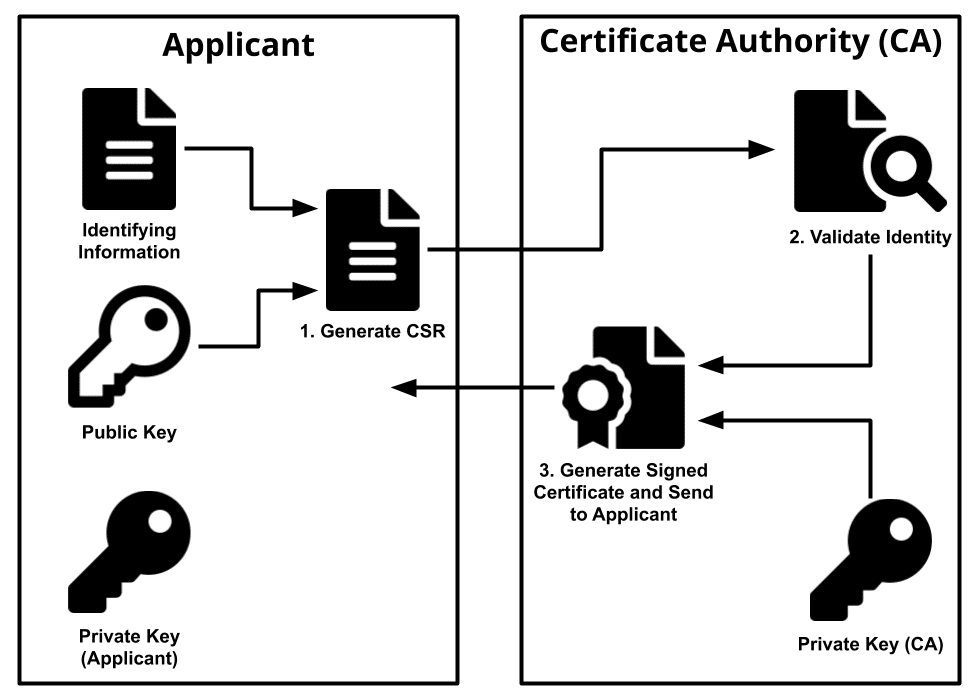
\includegraphics[width=0.6\textwidth]{ca-diagram.png}
        % \caption{Caption}
        % \label{fig:my_label}
    \end{figure}
\end{frame}

\begin{frame}{PKI in SSL/TLS}
    \begin{itemize}
        \item Domain Validation
        \item Organization Validation
        \item Extended Validation
    \end{itemize}
\end{frame}
\begin{frame}{PKI in SSL/TLS}
    \begin{columns}
        \begin{column}{0.25\textwidth}
            \begin{figure}
                \centering
                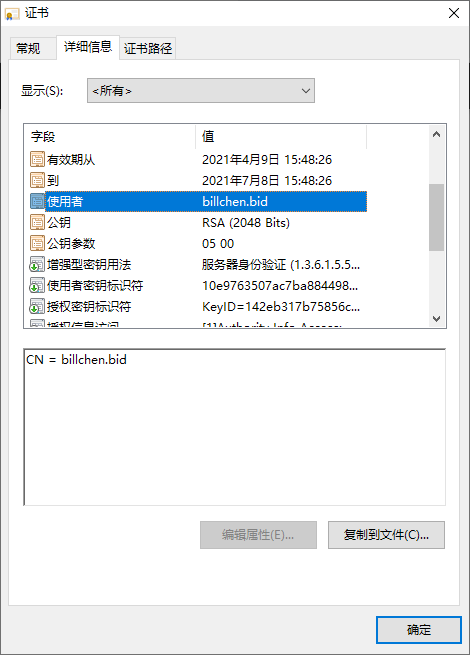
\includegraphics[width=\textwidth]{dv.png}
            \end{figure}
        \end{column}
        \begin{column}{0.25\textwidth}
            \begin{figure}
                \centering
                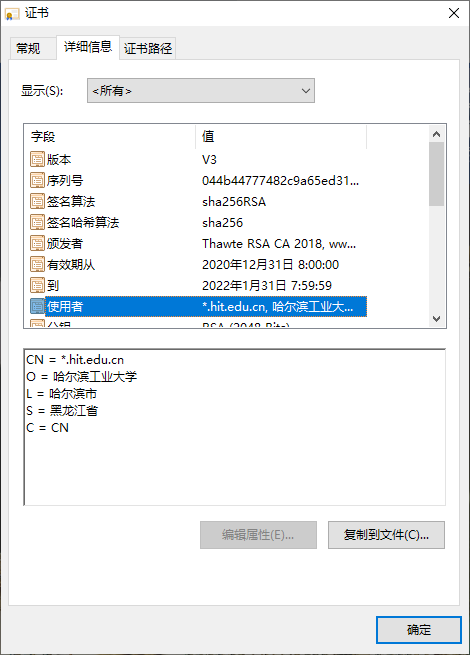
\includegraphics[width=\textwidth]{ov.png}
            \end{figure}
        \end{column}
        \begin{column}{0.25\textwidth}
            \begin{figure}
                \centering
                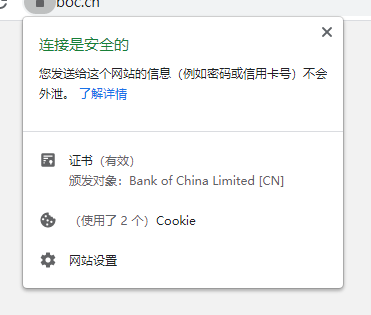
\includegraphics[width=0.8\textwidth]{ev-1.png}
            \end{figure}
            \begin{figure}
                \centering
                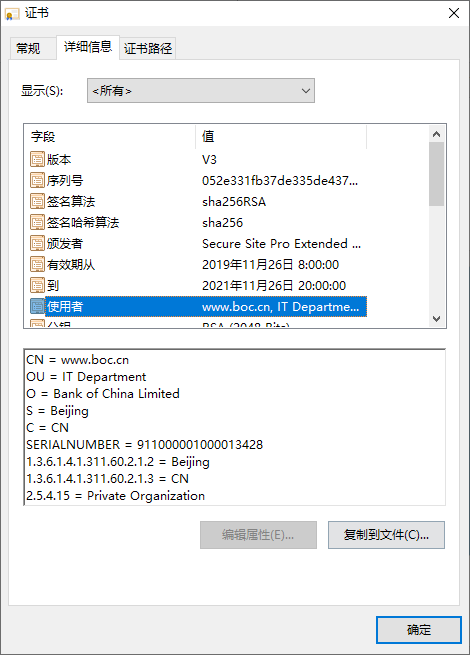
\includegraphics[width=\textwidth]{ev-2.png}
            \end{figure}
        \end{column}
    \end{columns}
\end{frame}

\begin{frame}{PKI in SSL/TLS}
    \begin{itemize}
        \item \textit{\href{https://datatracker.ietf.org/doc/html/rfc8555}{Automated Certificate Management} Environment(rfc8555)}
        \item ca-certificates
        \item Certificate revocation list (CRL)
        \item Online Certificate Status Protocol (OCSP)
    \end{itemize}
    
    \vspace{2em}
    
    \centering
    \textit{\url{https://crt.sh/}}
\end{frame}

\section{Applications}

\begin{frame}{Applications}
    \begin{itemize}
        \item SSH
        \item TLS
        \item PGP
        \item Blockchain
    \end{itemize}
\end{frame}

\subsection{SSH}
\begin{frame}{SSH}

    Secure SHell (protocol)
    
    \vspace{1em}
    
    Alternative to telnet
    
    Dropbear, OpenSSH, PuTTY
    
    \begin{itemize}
        \item Connect to remote server
        \item Port Forwarding
        \item X11 Forwarding
        \item SFTP / SCP
    \end{itemize}
    
    Push Git commit to \textit{\href{https://docs.github.com/en/github/authenticating-to-github/connecting-to-github-with-ssh}{GitHub}}, \textit{\href{https://docs.gitlab.com/ee/ssh/}{GitLab}}
\end{frame}

\subsection{TLS}
\begin{frame}{TLS}
    BoringSSL, GnuTLS, LibreSSL, OpenSSL, wolfSSL
    
    \vspace{1em}
    
    \begin{itemize}
        \item HTTPS
        \item Email
        \item FTPS
        \item DNS
        \item mmTLS
    \end{itemize}
\end{frame}

\subsection{PGP}
\begin{frame}{PGP}
    Pretty Good Privacy
    
    GnuPG, GnuPG2
    
    \begin{itemize}
        \item apt, rpm, pacman
        \item email
        \item \textit{\href{https://docs.github.com/en/github/authenticating-to-github/managing-commit-signature-verification}{Git Commit, Git Tag}}
        \item XMPP
    \end{itemize}
\end{frame}

\begin{frame}{PGP}
    Key server

    \vspace{1em}
    
    \begin{itemize}
        \item keys.openpgp.org
        \item pgp.mit.edu
        \item keyring.debian.org
        \item keyserver.ubuntu.com
        \item attester.flowcrypt.com
        \item zimmermann.mayfirst.org
    \end{itemize}
    
\end{frame}

\subsection{BlockChain}
\begin{frame}{BlockChain}

    BTC: Bitcoin uses the Elliptic Curve Digital Signature Algorithm (ECDSA). Your private key is used to create the signature and your public key is used to verify the signature.
    
    \vspace{1em}
    
    ETH: Ethereum uses ECDSA (Elliptic Curve Digital Signature Algorithm) for it's public-key cryptography.
    
    \begin{figure}
        \centering
        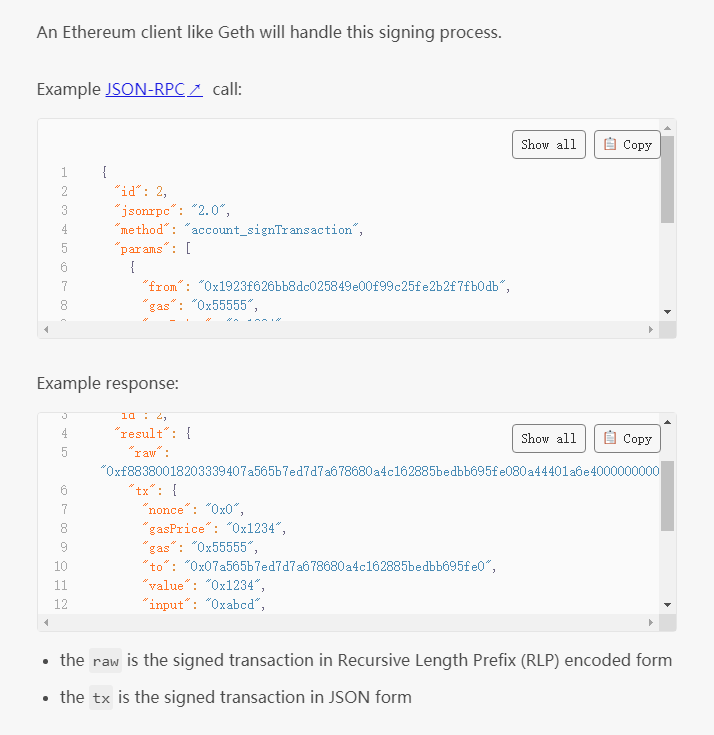
\includegraphics[width=0.35\textwidth]{eth.png}
    \end{figure}
\end{frame}

\section{Key signing Party}
\begin{frame}{Key signing Party}
    \begin{figure}
        \centering
        
\includegraphics[width=0.4\textwidth]{gnupg.png}
    \end{figure}
\end{frame}

\begin{frame}{Key signing Party}
    \begin{itemize}
        \item Create a keypair
        \item Generate a revocation certificate
        \item Make your public key public
        \item Get your key digitally signed
        \item Send your signed key to the server
    \end{itemize}
    
    \vspace{1em}
    
    \textit{\url{https://wiki.debian.org/Keysigning}}
    
    \textit{\url{https://wiki.ubuntu.com/KeySigningParty}}
    
    \textit{\href{https://cryptnet.net/fdp/crypto/keysigning_party/en/keysigning_party.html}{The Keysigning Party HOWTO}}
\end{frame}

\end{document}
